\documentclass[12pt]{article}
\usepackage[table]{xcolor}
\usepackage[shortlabels]{enumitem}
\usepackage{tabularx,xltabular}
\usepackage{graphicx}
\usepackage{hyperref}
\usepackage{verbatim}
\usepackage{geometry}
\usepackage{ulem}
\usepackage[official]{eurosym}
\usepackage{tikz}
\usetikzlibrary{arrows,backgrounds,calc,decorations.markings,patterns,3d,positioning,fit,angles, quotes}
\usepackage{pgfplots}
\pgfplotsset{compat = newest}
\usetikzlibrary{fit}
\newcommand\addvmargin[1]{
\usetikzlibrary{arrows}
\node[fit=(current bounding box),inner ysep=#1,inner xsep=0]{};}
\usepackage{cancel}
\usepackage{fontspec}
\usepackage{array}  
\geometry{a4paper, top=2cm, left=2cm, right=2cm, bottom=2cm, headsep=1cm}
\usepackage{tabu}
\usepackage{pst-node}
\usepackage{colortbl}
\usepackage{array}
\usepackage{german}
\setlength\parindent{0pt}
\newcolumntype{?}{!{\vrule width 1pt}}
\usepackage{makecell}
\renewcommand{\arraystretch}{2.5}
\usepackage{pbox}
\usepackage{amssymb}
\usepackage{amsmath}
\usepackage{booktabs}
\newcolumntype{L}[1]{>{\raggedright\let\newline\\\arraybackslash\hspace{0pt}}m{#1}}
\newcolumntype{C}[1]{>{\centering\let\newline\\\arraybackslash\hspace{0pt}}m{#1}}
\newcolumntype{R}[1]{>{\raggedleft\let\newline\\\arraybackslash\hspace{0pt}}m{#1}}
\begin{document}
\rightline{Datum: 08.12.2023}
\centerline{{\Large Tägliche Übungen}} 
\vspace{1cm}
\noindent \\


\begin{xltabular}{\textwidth}{|C{0.75cm}|X|C{0.75cm}|X|}
\arrayrulecolor{black}\hline
a)&\pbox{5cm}{
Berechne den Flächeninhalt von:\\
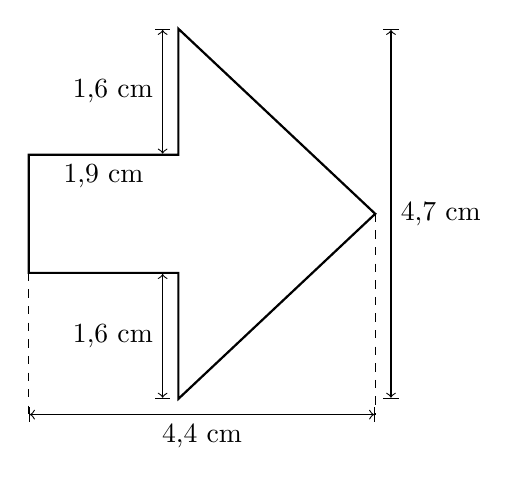
\begin{tikzpicture}
\draw[thick] (0,0) coordinate(A)-- ++(1.9,0)coordinate(B) -- ++(0,-1.6)coordinate(C) -- ++(2.5,2.35)coordinate(D) -- ++(-2.5,2.35)coordinate(E) -- ++(0,-1.6)coordinate(F) -- ++(-1.9,0)coordinate(G) -- cycle; 
\node[below] at ($(G)!0.5!(F)$){1,9 cm} ;
\draw[|<->|] (0,-1.8) -- node[below] {4,4 cm} ++(4.4,0);
\draw[dashed]  (A) -- ++(0,-1.8) ;
\draw[dashed]  (D) -- ++(0,-2.5500000000000003) ;
\draw[|<->|] (4.6000000000000005,-1.6) -- node[right] {4,7 cm} ++(0,4.7);
\draw[|<->|] (1.7,-1.6) -- node[left] {1,6 cm} ++(0,1.6);
\draw[|<->|] (1.7,1.5) -- node[left] {1,6 cm} ++(0,1.6);
\end{tikzpicture}
}
&
b)&\pbox{5cm}{
Berechne den Flächeninhalt von:\\
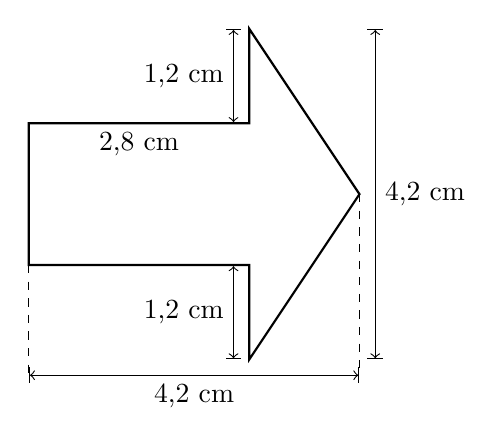
\begin{tikzpicture}
\draw[thick] (0,0) coordinate(A)-- ++(2.8,0)coordinate(B) -- ++(0,-1.2)coordinate(C) -- ++(1.4,2.1)coordinate(D) -- ++(-1.4,2.1)coordinate(E) -- ++(0,-1.2)coordinate(F) -- ++(-2.8,0)coordinate(G) -- cycle; 
\node[below] at ($(G)!0.5!(F)$){2,8 cm} ;
\draw[|<->|] (0,-1.4) -- node[below] {4,2 cm} ++(4.199999999999999,0);
\draw[dashed]  (A) -- ++(0,-1.4) ;
\draw[dashed]  (D) -- ++(0,-2.3000000000000003) ;
\draw[|<->|] (4.3999999999999995,-1.2) -- node[right] {4,2 cm} ++(0,4.2);
\draw[|<->|] (2.5999999999999996,-1.2) -- node[left] {1,2 cm} ++(0,1.2);
\draw[|<->|] (2.5999999999999996,1.8000000000000003) -- node[left] {1,2 cm} ++(0,1.2);
\end{tikzpicture}
}
\\\hline
c)&\pbox{5cm}{
Berechne den Flächeninhalt von:\\
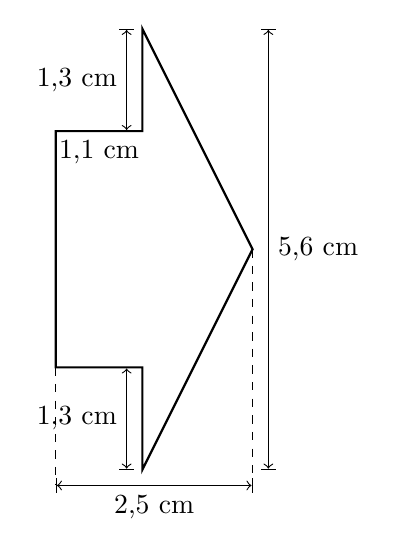
\begin{tikzpicture}
\draw[thick] (0,0) coordinate(A)-- ++(1.1,0)coordinate(B) -- ++(0,-1.3)coordinate(C) -- ++(1.4,2.8)coordinate(D) -- ++(-1.4,2.8)coordinate(E) -- ++(0,-1.3)coordinate(F) -- ++(-1.1,0)coordinate(G) -- cycle; 
\node[below] at ($(G)!0.5!(F)$){1,1 cm} ;
\draw[|<->|] (0,-1.5) -- node[below] {2,5 cm} ++(2.5,0);
\draw[dashed]  (A) -- ++(0,-1.5) ;
\draw[dashed]  (D) -- ++(0,-3.0) ;
\draw[|<->|] (2.7,-1.3) -- node[right] {5,6 cm} ++(0,5.6);
\draw[|<->|] (0.9000000000000001,-1.3) -- node[left] {1,3 cm} ++(0,1.3);
\draw[|<->|] (0.9000000000000001,2.9999999999999996) -- node[left] {1,3 cm} ++(0,1.3);
\end{tikzpicture}
}
&
d)&\pbox{5cm}{
Berechne den Flächeninhalt von:\\
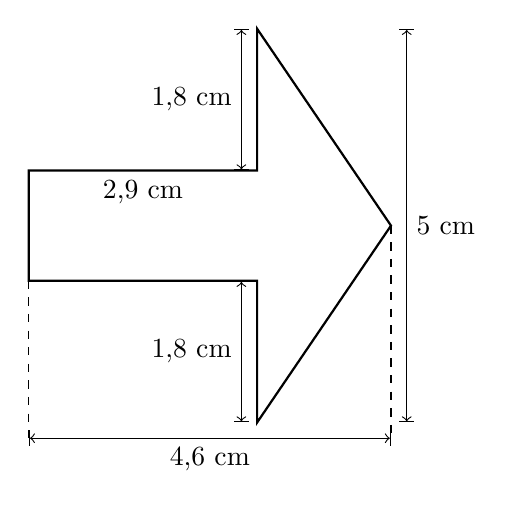
\begin{tikzpicture}
\draw[thick] (0,0) coordinate(A)-- ++(2.9,0)coordinate(B) -- ++(0,-1.8)coordinate(C) -- ++(1.7,2.5)coordinate(D) -- ++(-1.7,2.5)coordinate(E) -- ++(0,-1.8)coordinate(F) -- ++(-2.9,0)coordinate(G) -- cycle; 
\node[below] at ($(G)!0.5!(F)$){2,9 cm} ;
\draw[|<->|] (0,-2.0) -- node[below] {4,6 cm} ++(4.6,0);
\draw[dashed]  (A) -- ++(0,-2.0) ;
\draw[dashed]  (D) -- ++(0,-2.7) ;
\draw[|<->|] (4.8,-1.8) -- node[right] {5 cm} ++(0,5.0);
\draw[|<->|] (2.6999999999999997,-1.8) -- node[left] {1,8 cm} ++(0,1.8);
\draw[|<->|] (2.6999999999999997,1.4) -- node[left] {1,8 cm} ++(0,1.8);
\end{tikzpicture}
}
\\\hline
e)&\pbox{5cm}{
Berechne den Flächeninhalt von:\\
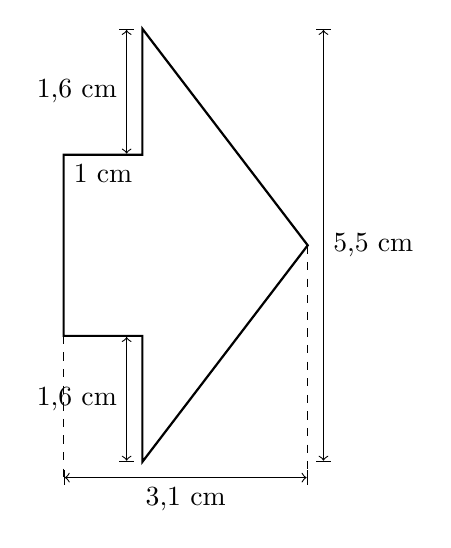
\begin{tikzpicture}
\draw[thick] (0,0) coordinate(A)-- ++(1.0,0)coordinate(B) -- ++(0,-1.6)coordinate(C) -- ++(2.1,2.75)coordinate(D) -- ++(-2.1,2.75)coordinate(E) -- ++(0,-1.6)coordinate(F) -- ++(-1.0,0)coordinate(G) -- cycle; 
\node[below] at ($(G)!0.5!(F)$){1 cm} ;
\draw[|<->|] (0,-1.8) -- node[below] {3,1 cm} ++(3.1,0);
\draw[dashed]  (A) -- ++(0,-1.8) ;
\draw[dashed]  (D) -- ++(0,-2.95) ;
\draw[|<->|] (3.3000000000000003,-1.6) -- node[right] {5,5 cm} ++(0,5.5);
\draw[|<->|] (0.8,-1.6) -- node[left] {1,6 cm} ++(0,1.6);
\draw[|<->|] (0.8,2.3) -- node[left] {1,6 cm} ++(0,1.6);
\end{tikzpicture}
}
&
f)&\pbox{5cm}{
Berechne den Flächeninhalt von:\\
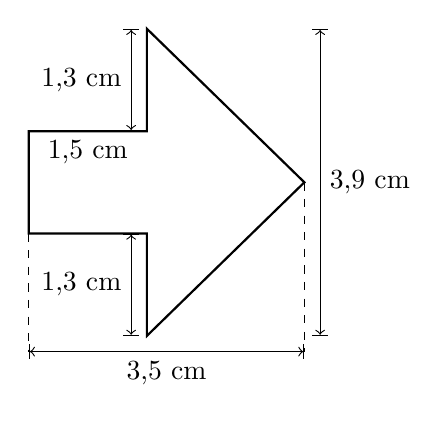
\begin{tikzpicture}
\draw[thick] (0,0) coordinate(A)-- ++(1.5,0)coordinate(B) -- ++(0,-1.3)coordinate(C) -- ++(2.0,1.9500000000000002)coordinate(D) -- ++(-2.0,1.9500000000000002)coordinate(E) -- ++(0,-1.3)coordinate(F) -- ++(-1.5,0)coordinate(G) -- cycle; 
\node[below] at ($(G)!0.5!(F)$){1,5 cm} ;
\draw[|<->|] (0,-1.5) -- node[below] {3,5 cm} ++(3.5,0);
\draw[dashed]  (A) -- ++(0,-1.5) ;
\draw[dashed]  (D) -- ++(0,-2.1500000000000004) ;
\draw[|<->|] (3.7,-1.3) -- node[right] {3,9 cm} ++(0,3.9000000000000004);
\draw[|<->|] (1.3,-1.3) -- node[left] {1,3 cm} ++(0,1.3);
\draw[|<->|] (1.3,1.3000000000000003) -- node[left] {1,3 cm} ++(0,1.3);
\end{tikzpicture}
}
\\\hline
\end{xltabular}
\vspace{0.5cm}
\newpage
\rightline{Datum: 08.12.2023}
\centerline{{\large Lösungen Tägliche Übungen}} 
\vspace{0.5cm}

\begin{xltabular}{\textwidth}{|C{0.75cm}|X|C{0.75cm}|X|}
\arrayrulecolor{black}\hline
a)&\pbox{7cm}{
\tikzstyle{background grid}=[draw, black!15,step=.5cm]
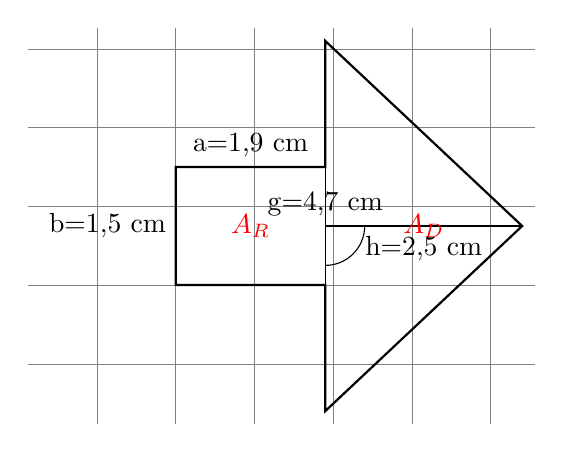
\begin{tikzpicture}[show background grid]
\draw[thick] (0,0) coordinate(A)-- ++(1.9,0)coordinate(B) -- ++(0,-1.6)coordinate(C) -- ++(2.5,2.35)coordinate(D) -- ++(-2.5,2.35)coordinate(E) -- ++(0,-1.6)coordinate(F) -- ++(-1.9,0)coordinate(G) -- cycle; 
\node[above] at ($(G)!0.5!(F)$){a=1,9 cm} ;
\draw (C) --node[above] {g=4,7 cm} (E);
\draw (D) --node[below] {h=2,5 cm} ++(-2.5,0) coordinate(H);
\pic [draw, -,angle radius=0.5cm] {angle = B--H--D};
\node[left] at ($(A)!0.5!(G)$){b=1,5 cm} ;
\node[red] at ($(A)!0.5!(F)$) {$A_R$};
\node[red] at ($(H)!0.5!(D)$) {$A_D$};
\end{tikzpicture}
\\
$\begin{aligned}
geg.: a &=1,9~cm& & \\
  b &=1,5~cm& & \\
  g &=4,7~cm& & \\
  h &=2,5~cm& & \\
ges.: A_G &=?~cm^2& & \\
& & & \\
A_G&= A_R+A_D & & \\
A_R&= a \cdot b & & \\
\makebox[0pt][l]{\uline{\phantom{$A_R= 1,9 \cdot 1,5=2,85cm^2   \\$} } }
A_R&= 1,9 \cdot 1,5=2,85cm^2 & & \\
A_D&= \frac{g\cdot h}{2} & & \\
\makebox(0pt,-0.25cm)[l]{\uline{\phantom{$A_D= \frac{4,7\cdot 2,5}{2} =5,875 cm^2  \\$} } }
A_D&= \frac{4,7\cdot 2,5}{2} =5,875 cm^2& & \\
\makebox[0pt][l]{\uuline{\phantom{$A_G= A_R+A_D=2,85+5,875=8,725 cm ^2  \\$} } }
A_G&= A_R+A_D=2,85+5,875=8,725 cm ^2& & \\
\end{aligned}$
}
&
b)&\pbox{7cm}{
\tikzstyle{background grid}=[draw, black!15,step=.5cm]
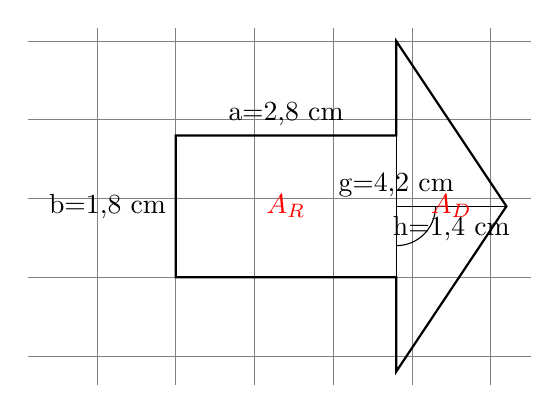
\begin{tikzpicture}[show background grid]
\draw[thick] (0,0) coordinate(A)-- ++(2.8,0)coordinate(B) -- ++(0,-1.2)coordinate(C) -- ++(1.4,2.1)coordinate(D) -- ++(-1.4,2.1)coordinate(E) -- ++(0,-1.2)coordinate(F) -- ++(-2.8,0)coordinate(G) -- cycle; 
\node[above] at ($(G)!0.5!(F)$){a=2,8 cm} ;
\draw (C) --node[above] {g=4,2 cm} (E);
\draw (D) --node[below] {h=1,4 cm} ++(-1.4,0) coordinate(H);
\pic [draw, -,angle radius=0.5cm] {angle = B--H--D};
\node[left] at ($(A)!0.5!(G)$){b=1,8 cm} ;
\node[red] at ($(A)!0.5!(F)$) {$A_R$};
\node[red] at ($(H)!0.5!(D)$) {$A_D$};
\end{tikzpicture}
\\
$\begin{aligned}
geg.: a &=2,8~cm& & \\
  b &=1,8~cm& & \\
  g &=4,2~cm& & \\
  h &=1,4~cm& & \\
ges.: A_G &=?~cm^2& & \\
& & & \\
A_G&= A_R+A_D & & \\
A_R&= a \cdot b & & \\
\makebox[0pt][l]{\uline{\phantom{$A_R= 2,8 \cdot 1,8=5,04cm^2   \\$} } }
A_R&= 2,8 \cdot 1,8=5,04cm^2 & & \\
A_D&= \frac{g\cdot h}{2} & & \\
\makebox(0pt,-0.25cm)[l]{\uline{\phantom{$A_D= \frac{4,2\cdot 1,4}{2} =2,94 cm^2  \\$} } }
A_D&= \frac{4,2\cdot 1,4}{2} =2,94 cm^2& & \\
\makebox[0pt][l]{\uuline{\phantom{$A_G= A_R+A_D=5,04+2,94=7,98 cm ^2  \\$} } }
A_G&= A_R+A_D=5,04+2,94=7,98 cm ^2& & \\
\end{aligned}$
}
\\\hline
c)&\pbox{7cm}{
\tikzstyle{background grid}=[draw, black!15,step=.5cm]
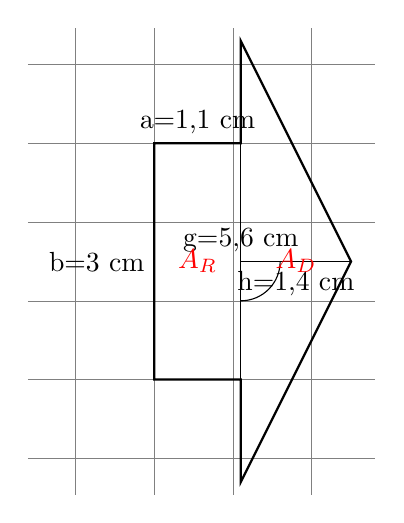
\begin{tikzpicture}[show background grid]
\draw[thick] (0,0) coordinate(A)-- ++(1.1,0)coordinate(B) -- ++(0,-1.3)coordinate(C) -- ++(1.4,2.8)coordinate(D) -- ++(-1.4,2.8)coordinate(E) -- ++(0,-1.3)coordinate(F) -- ++(-1.1,0)coordinate(G) -- cycle; 
\node[above] at ($(G)!0.5!(F)$){a=1,1 cm} ;
\draw (C) --node[above] {g=5,6 cm} (E);
\draw (D) --node[below] {h=1,4 cm} ++(-1.4,0) coordinate(H);
\pic [draw, -,angle radius=0.5cm] {angle = B--H--D};
\node[left] at ($(A)!0.5!(G)$){b=3 cm} ;
\node[red] at ($(A)!0.5!(F)$) {$A_R$};
\node[red] at ($(H)!0.5!(D)$) {$A_D$};
\end{tikzpicture}
\\
$\begin{aligned}
geg.: a &=1,1~cm& & \\
  b &=3~cm& & \\
  g &=5,6~cm& & \\
  h &=1,4~cm& & \\
ges.: A_G &=?~cm^2& & \\
& & & \\
A_G&= A_R+A_D & & \\
A_R&= a \cdot b & & \\
\makebox[0pt][l]{\uline{\phantom{$A_R= 1,1 \cdot 3=3,3cm^2   \\$} } }
A_R&= 1,1 \cdot 3=3,3cm^2 & & \\
A_D&= \frac{g\cdot h}{2} & & \\
\makebox(0pt,-0.25cm)[l]{\uline{\phantom{$A_D= \frac{5,6\cdot 1,4}{2} =3,92 cm^2  \\$} } }
A_D&= \frac{5,6\cdot 1,4}{2} =3,92 cm^2& & \\
\makebox[0pt][l]{\uuline{\phantom{$A_G= A_R+A_D=3,3+3,92=7,22 cm ^2  \\$} } }
A_G&= A_R+A_D=3,3+3,92=7,22 cm ^2& & \\
\end{aligned}$
}
&
d)&\pbox{7cm}{
\tikzstyle{background grid}=[draw, black!15,step=.5cm]
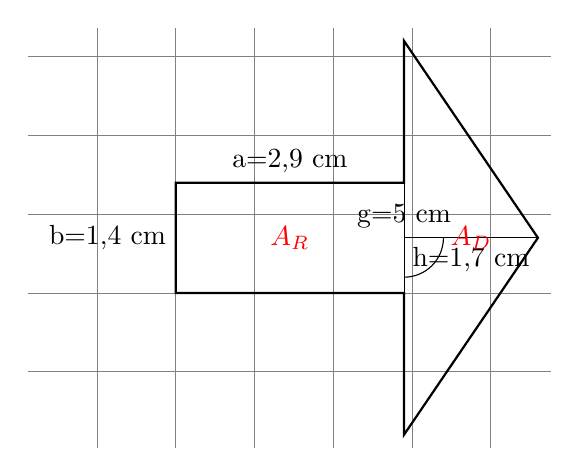
\begin{tikzpicture}[show background grid]
\draw[thick] (0,0) coordinate(A)-- ++(2.9,0)coordinate(B) -- ++(0,-1.8)coordinate(C) -- ++(1.7,2.5)coordinate(D) -- ++(-1.7,2.5)coordinate(E) -- ++(0,-1.8)coordinate(F) -- ++(-2.9,0)coordinate(G) -- cycle; 
\node[above] at ($(G)!0.5!(F)$){a=2,9 cm} ;
\draw (C) --node[above] {g=5 cm} (E);
\draw (D) --node[below] {h=1,7 cm} ++(-1.7,0) coordinate(H);
\pic [draw, -,angle radius=0.5cm] {angle = B--H--D};
\node[left] at ($(A)!0.5!(G)$){b=1,4 cm} ;
\node[red] at ($(A)!0.5!(F)$) {$A_R$};
\node[red] at ($(H)!0.5!(D)$) {$A_D$};
\end{tikzpicture}
\\
$\begin{aligned}
geg.: a &=2,9~cm& & \\
  b &=1,4~cm& & \\
  g &=5~cm& & \\
  h &=1,7~cm& & \\
ges.: A_G &=?~cm^2& & \\
& & & \\
A_G&= A_R+A_D & & \\
A_R&= a \cdot b & & \\
\makebox[0pt][l]{\uline{\phantom{$A_R= 2,9 \cdot 1,4=4,06cm^2   \\$} } }
A_R&= 2,9 \cdot 1,4=4,06cm^2 & & \\
A_D&= \frac{g\cdot h}{2} & & \\
\makebox(0pt,-0.25cm)[l]{\uline{\phantom{$A_D= \frac{5\cdot 1,7}{2} =4,25 cm^2  \\$} } }
A_D&= \frac{5\cdot 1,7}{2} =4,25 cm^2& & \\
\makebox[0pt][l]{\uuline{\phantom{$A_G= A_R+A_D=4,06+4,25=8,31 cm ^2  \\$} } }
A_G&= A_R+A_D=4,06+4,25=8,31 cm ^2& & \\
\end{aligned}$
}
\\\hline
e)&\pbox{7cm}{
\tikzstyle{background grid}=[draw, black!15,step=.5cm]
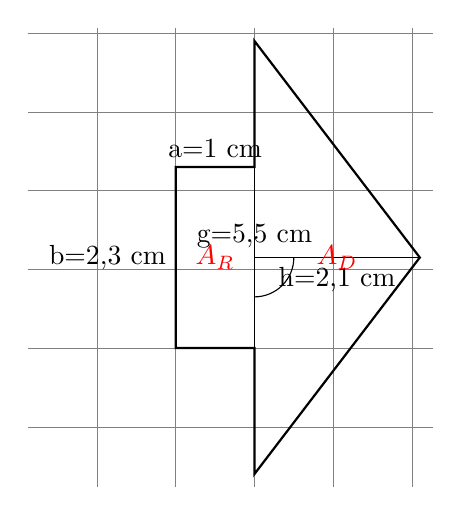
\begin{tikzpicture}[show background grid]
\draw[thick] (0,0) coordinate(A)-- ++(1.0,0)coordinate(B) -- ++(0,-1.6)coordinate(C) -- ++(2.1,2.75)coordinate(D) -- ++(-2.1,2.75)coordinate(E) -- ++(0,-1.6)coordinate(F) -- ++(-1.0,0)coordinate(G) -- cycle; 
\node[above] at ($(G)!0.5!(F)$){a=1 cm} ;
\draw (C) --node[above] {g=5,5 cm} (E);
\draw (D) --node[below] {h=2,1 cm} ++(-2.1,0) coordinate(H);
\pic [draw, -,angle radius=0.5cm] {angle = B--H--D};
\node[left] at ($(A)!0.5!(G)$){b=2,3 cm} ;
\node[red] at ($(A)!0.5!(F)$) {$A_R$};
\node[red] at ($(H)!0.5!(D)$) {$A_D$};
\end{tikzpicture}
\\
$\begin{aligned}
geg.: a &=1~cm& & \\
  b &=2,3~cm& & \\
  g &=5,5~cm& & \\
  h &=2,1~cm& & \\
ges.: A_G &=?~cm^2& & \\
& & & \\
A_G&= A_R+A_D & & \\
A_R&= a \cdot b & & \\
\makebox[0pt][l]{\uline{\phantom{$A_R= 1 \cdot 2,3=2,3cm^2   \\$} } }
A_R&= 1 \cdot 2,3=2,3cm^2 & & \\
A_D&= \frac{g\cdot h}{2} & & \\
\makebox(0pt,-0.25cm)[l]{\uline{\phantom{$A_D= \frac{5,5\cdot 2,1}{2} =5,775 cm^2  \\$} } }
A_D&= \frac{5,5\cdot 2,1}{2} =5,775 cm^2& & \\
\makebox[0pt][l]{\uuline{\phantom{$A_G= A_R+A_D=2,3+5,775=8,075 cm ^2  \\$} } }
A_G&= A_R+A_D=2,3+5,775=8,075 cm ^2& & \\
\end{aligned}$
}
&
f)&\pbox{7cm}{
\tikzstyle{background grid}=[draw, black!15,step=.5cm]
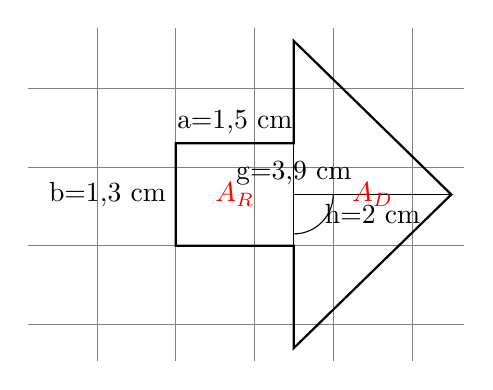
\begin{tikzpicture}[show background grid]
\draw[thick] (0,0) coordinate(A)-- ++(1.5,0)coordinate(B) -- ++(0,-1.3)coordinate(C) -- ++(2.0,1.9500000000000002)coordinate(D) -- ++(-2.0,1.9500000000000002)coordinate(E) -- ++(0,-1.3)coordinate(F) -- ++(-1.5,0)coordinate(G) -- cycle; 
\node[above] at ($(G)!0.5!(F)$){a=1,5 cm} ;
\draw (C) --node[above] {g=3,9 cm} (E);
\draw (D) --node[below] {h=2 cm} ++(-2.0,0) coordinate(H);
\pic [draw, -,angle radius=0.5cm] {angle = B--H--D};
\node[left] at ($(A)!0.5!(G)$){b=1,3 cm} ;
\node[red] at ($(A)!0.5!(F)$) {$A_R$};
\node[red] at ($(H)!0.5!(D)$) {$A_D$};
\end{tikzpicture}
\\
$\begin{aligned}
geg.: a &=1,5~cm& & \\
  b &=1,3~cm& & \\
  g &=3,9~cm& & \\
  h &=2~cm& & \\
ges.: A_G &=?~cm^2& & \\
& & & \\
A_G&= A_R+A_D & & \\
A_R&= a \cdot b & & \\
\makebox[0pt][l]{\uline{\phantom{$A_R= 1,5 \cdot 1,3=1,95cm^2   \\$} } }
A_R&= 1,5 \cdot 1,3=1,95cm^2 & & \\
A_D&= \frac{g\cdot h}{2} & & \\
\makebox(0pt,-0.25cm)[l]{\uline{\phantom{$A_D= \frac{3,9\cdot 2}{2} =3,9 cm^2  \\$} } }
A_D&= \frac{3,9\cdot 2}{2} =3,9 cm^2& & \\
\makebox[0pt][l]{\uuline{\phantom{$A_G= A_R+A_D=1,95+3,9=5,85 cm ^2  \\$} } }
A_G&= A_R+A_D=1,95+3,9=5,85 cm ^2& & \\
\end{aligned}$
}
\\\hline
\end{xltabular}
\vspace{0.5cm}
\end{document}